\documentclass[runningheads,a4paper]{llncs}
% \documentclass{article}
\usepackage{amssymb}
\usepackage{amsmath}
\setcounter{tocdepth}{3}
\usepackage{graphicx}
\usepackage{url}
\usepackage[algoruled, vlined,linesnumbered]{algorithm2e}
\usepackage{color}

\begin{document}

\mainmatter 

\title{Autonomous Realization of Simple Machines}
\author{Can Erdogan \and Mike Stilman}
\institute{Institute for Robotics and Intelligent Machines \\Georgia Institute of Technology}
\maketitle

\begin{abstract}

For robots to become integral parts of human daily experi- ence, they need to be able to utilize the
objects in their environment to accomplish any range of tasks. In this work, we focus particularly
on physically challenging tasks that push the limits on the robot kinodynamic constraints such as
joint limits, joint torques and etc. Previously, we demonstrated an autonomous planner that
instructs a human collab- orator where to place the available objects in the environment to form a
simple machine such as a lever-fulcrum assembly. In this work, we report results on the autonomous
realization of such a design by the humanoid robot Golem Krang, focusing on the challenges of
autonomous perception, manipulation and control.

\end{abstract}

\section{Introduction}

The ability to use the available objects in the environment towards accomplishing goals is essential
to thriving in challenging circumstances. Everyday examples of tool use include simple machines such
as levers and pulleys. The challenge in autonomous design of such simple machines is the space of
discrete choices for the component options and the related high-dimensional continuous configuration
space of the chosen components.

In previous work \cite{erdogan2013planning} \cite{erdogan2014incorporating}, we demonstrated the
constraint satisfaction approach to assembly design, specifically for robotic manipulation and
locomotion. The key idea is to represent the constraints
between the components of the design, the robot kinematics and dynamics as generic equality and
inequality functions within a nonlinear optimization framework and solve for the global minima, if
 necessary by random restarts. Such global optimization methods have been used in other fields as
well, such as operations research \cite{vidal2006branching} and architecture \cite{yu2011make}.

In this work, we take the next step towards full autonomy where the humanoid robot, Golem Krang,
autonomously manipulates the objects in its environment to construct a simple machine. We present
an autonomous planner that perceives the available objects, specifically 15 kg cinder blocks and 10
kg 2-by-4 block blocks (e.g. potential levers), relocates them to the desired configurations output
by the constraint planner, and actuates them to flip a 50 kg load. Figure \ref{fig:showOff} demonstrates key scenes
from this scenario such as (a) detection of a cinder block, (b) locomotion with a heavy load, (c)
manipulating a lever while subject to multiple constraints and (d) application of force to the lever
leading to a successful load motion.

\begin{figure}[ht!] 
  \centering
  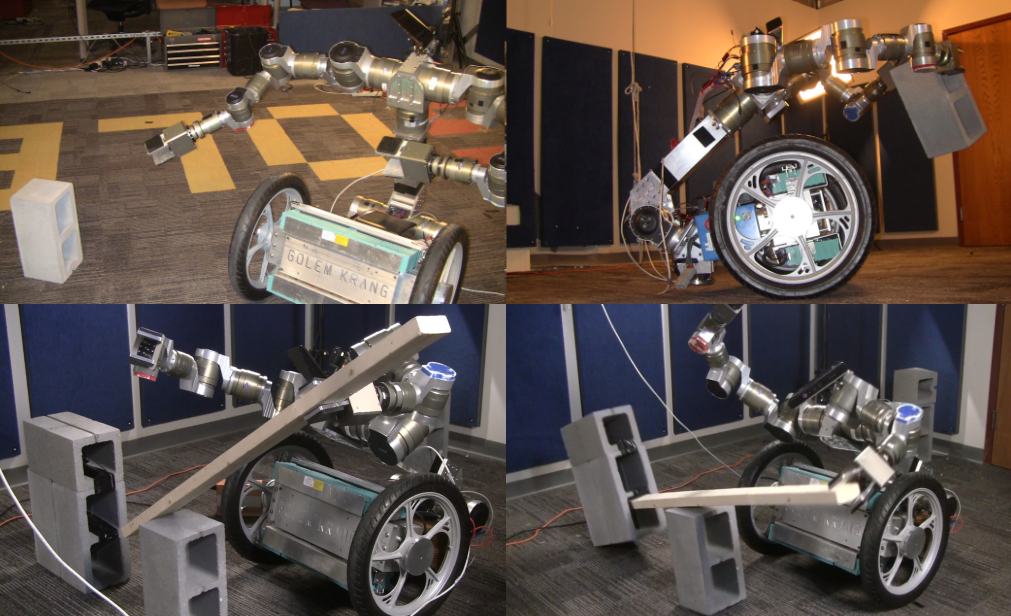
\includegraphics[width=1.0\linewidth]{Figures/showOff.png}
  \caption{The mechanical advantage in forces}
  \label{fig:showOff}
\end{figure}

Significant effort has been demonstrated by \cite{beetz2010cram} \cite{stilman2005navigation}
\cite{kemp2007challenges} to incorporate autonomous agents in human environments. Our work stands
out in multiple aspects from the established state of the art. First, Golem Krang is a two-wheeled
balancing robot, similar to a segway with two 7-dof robotic arms installed. The challenge with
such a platform is the dynamic stability constraint where the robot has to ensure its center of mass
is close to the wheel axis at all times as opposed to legged or multi-wheeled platforms. Secondly, to the best of our knowledge,
Golem Krang is the tallest and heaviest two-wheeled robot with 150 kg at 1.9 m, a unique property
among similar designs \cite{kuindersma2009dexterous}. As we expand in Section IV, at this scale, the
weight can help with heavy-duty manipulation but complicates the autonomous locomotion of the
agent. Lastly, Golem Krang perceives its environment with an onboard RGBD sensor with two degrees
of freedom that are manipulated autonomously for gaze control. Autonomous perception and scene
recognition has only recently started to gather interest in the humanoid robotics field
\cite{srinivasa2010herb} \cite{nishiwaki2000design} as opposed to the long established motion
capture methods \cite{dasgupta1999making}.

\newpage
\section{Technical Approach}

\subsection{Constraint Satisfaction for Simple Machine Designs}

The manipulation of multiple objects to achieve a goal can be readily represented in a constraint
satisfaction paradigm where the constraints represent the relationships between the design
components. In this work, we focus on simple machine designs such as lever-fulcrum assemblies or
inclined planes that need to be structurally stable and provide mechanical leverage to their users.
Reasoning about such design criteria requires analysis of more detailed concepts such as center
of masses, robot kinodynamic constraints and physics principles. 

The process for an autonomous planner is composed of three steps. First, from the set of available objects
in the environment, it needs to choose a subset that will be incorporated in the structure. Second,
the structure components are assigned roles that designate how they should be put together - specifically,
the constraints that \textit{bind} one to another. Lastly, the planner needs to configure the objects
such that the role constraints and the general design criteria are satisfied. 

\subsubsection{Component Choices}

A completeness property for an autonomous planner for structural designs is a crucial advantage
for deployment in real-world circumstances (e.g. military or search-and-rescue operations). In
emergency situations, when physically challenging that requires creative reasoning about simple
machines usually arise, the ability to exhaustively search for all possible solutions and determine
if one exists is a critical advantage. Note that we assume every object is used only once in the 
structure as opposed to the agent changing the structure as its being used.

In choosing a set of design components, an autonomous planner needs to exhaustively search the 
entire \textit{finite} space of discrete assignments. In comparison to continuous choices, such as
object configurations, the discrete nature of the choices (i.e. in or out) makes such a search
feasible. Despite the finite space, it is challenging to evaluate
every alternative since there is still a combinational number of roles and infinite 
space of configurations to reason about.

To remedy the computational challenge, pruning strategies and heuristics are significant tools in
cutting back the search at the top level. For instance, in construction a lever-fulcrum design,
two wooden blocks of the same size (or approximately to a degree of confidence) can be categorized
under one class. Similarly, for loads that are known to be significantly heavier than a robot can
handle, the longer lever candidates might be priotized in the search process.

\subsubsection{Object Roles} 

Imagine a two-step stairs is needed to enable a swarm of rough-terrain vehicles, such as 
PackBots or RHexs \cite{yamauchi2004packbot,saranli2001rhex}, climb a window and survey a building, and some of them have robotic
arms that can stack box-like objects. The goal for a planner would be to choose three boxes and
stack two of them (e.g. box B on C) such that the swarm can first climb one step and then move on to
the two stack, until it reaches the window sill. 

In coming up with this solution, two types of choices need to made. First, among the three objects,
say A, B, and C, which object would constitute as the first step and which one would be at the top
in the second step needs to be decided. Secondly, to place the objects on the ground or on top of
another object, a base face needs to be chosen to clarify the object roles and to simplify the
representation of the constraints for the object configurations. Note that choosing a base 
in fact partitions the configuration space of the objects even before the design constraints
are considered to prune infeasible assignments.

The goal of the object roles is to specify (1) the relationship of a component with respect to
others, and (2) which of its face and edges are used in these connections. Figure \ref{fig:matches} 
\cite{erdogan2014incorporating} demonstrates some outcome assemblies with the triangle prism
object acting as fulcrum positioned on different base faces and in contact with the chosen lever
on various edges. Similarly, we observe that the lever can be used on at least two of its faces
(discounting symmetries) while it is still possible to find a feasible assembly. 

\begin{figure}[ht!] 
  \centering
  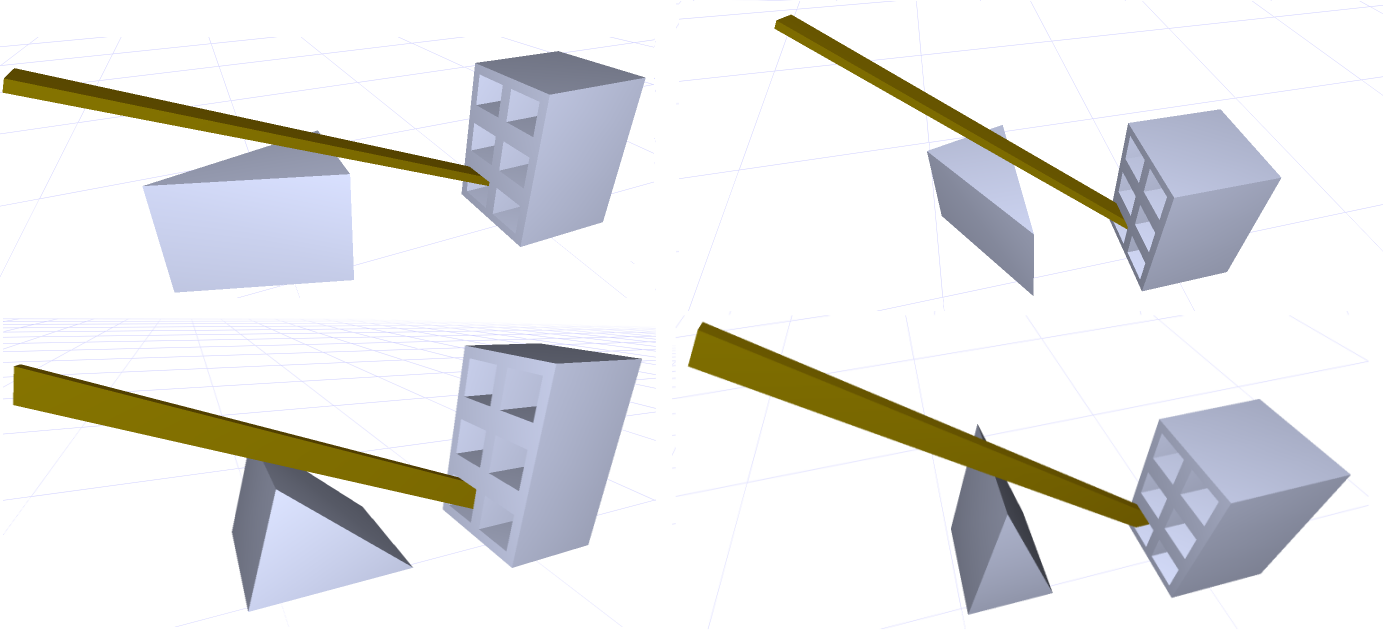
\includegraphics[width=0.7\linewidth]{Figures/matches.png}
  \caption{Different face and edge assignments for the lever-fulcrum assembly. Some assignments,
  such as using the shortest edge of the lever to connect the fulcrum and the load, may not
  be feasible due to design constraints and collisions.}
  \label{fig:matches}
\end{figure}

The role assignment to available resources has been a thoroughly studied area, starting from
classical planning \cite{newell1961gps,mccarthy1963programs}, and evolving into operations research
\cite{fulkerson1961network,taha1975integer}, and in this work, we adopt the STRIPS representation
for the planning process \cite{fikes1972strips}. The idea is to provide the domain knowledge of possible
actions to take on the available objects in the environment. For instance, a lever can be \textit{placed}
on a fulcrum or a ramp can be \textit{rested} against another object. A minor difference in our
framework is that every action induces additional constraints to the assembly configurations and
an action can be taken if and only if there exists some configuration that satisfies the accumulated
constraints.

\subsubsection{Continuous Configuration Space and Constraints}

The proposed framework accumulates design constraints via a classical planning framework
and a feasibility process determines whether the constraints can be satisfied by some configuration
of the components. The idea is that the different type of constraints can all be generically
expressed as equality or inequality functions on the space of object and robot configurations.
If all the constraints are convex, for instance in a stair or bridge design with simplified
robot assumptions, the feasibility can be determined by an efficient simplex algorithm
implementation \cite{erdogan2013planning}. For the larger set of nonconvex domains, especially when
robot kinodynamics are considered, we propose a nonlinear optimization process which minimizes the
violation of the constraints and attempts to find an assignment of configurations that satisfies all of them.

A number of design constraints such as stacking a box on top of another one or placing a lever
at the edge of a fulcrum can be expressed with geometric projections. Figure \ref{fig:constraints}
demonstrates three types of connections: (1) center of mass-face, (2) edge-face, and (3) face-face. 
The general idea is that points of interest such as center of mass, endpoints of an edge or vertices
of a face are projected to the plane of another face and limits are imposed on its location. For instance,
for two objects to be stacked successfully (A), the center of mass of the top object has to lie within
the supporting face of the bottom object. Similarly, to ensure an edge is on a face (B), it is sufficient
to confine the endpoints of the edge onto the face plane and guarantee there exists a shared point
(e.g. cross) between the edge and the face. Lastly, for contact between two faces (C), 
three points of one of the faces has to lie on the other one and again, a shared point should exist.
Observe that geometric contact concepts are easily expressed through equality
and inequality expressions on the projections of significant points on the meshes. 

\begin{figure}[ht!] 
  \centering
  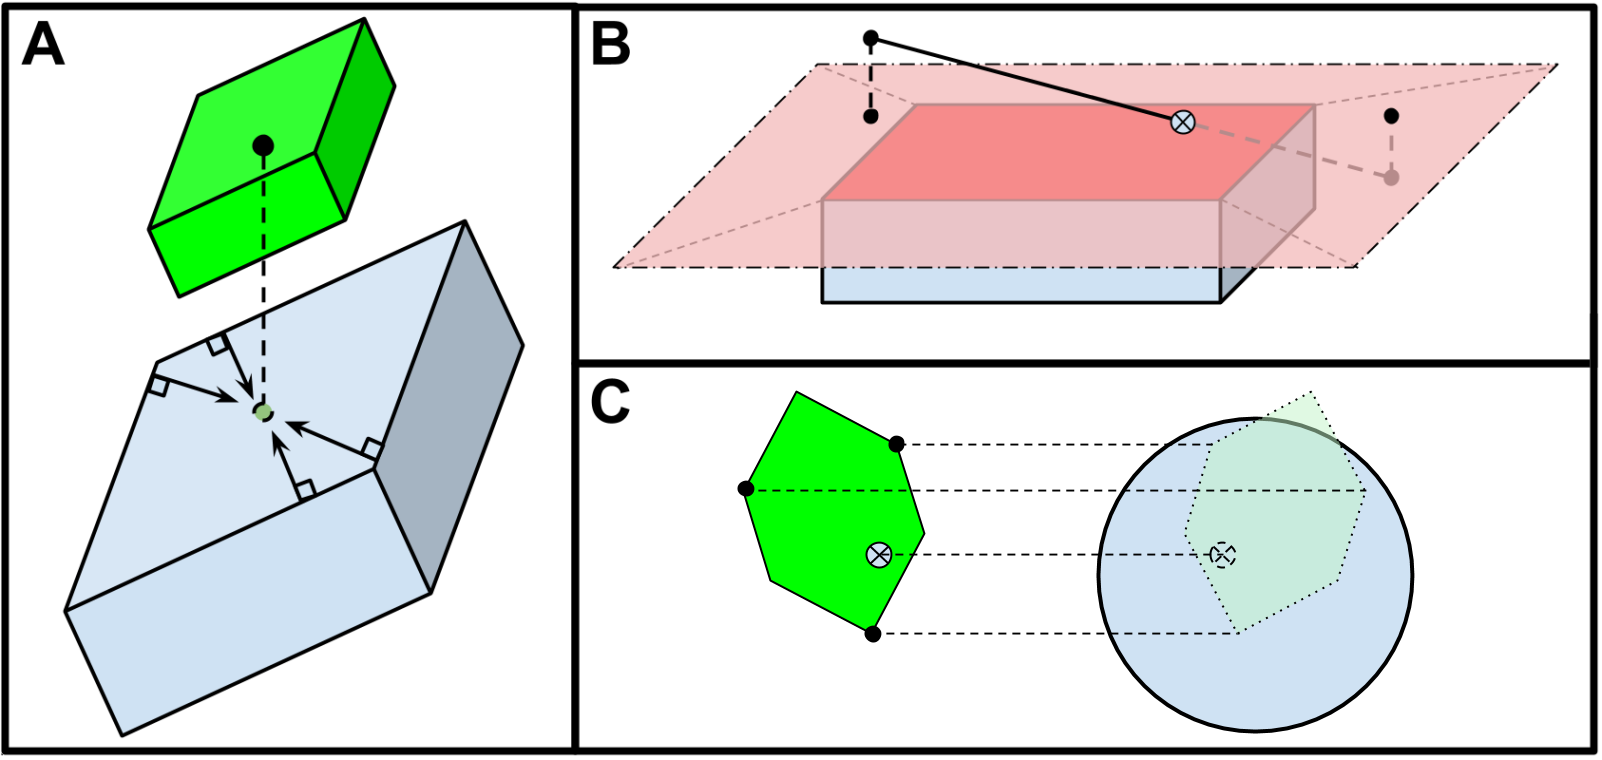
\includegraphics[width=0.75\linewidth]{Figures/constraints.png}
  \caption{Visualization of different types of geometric contact constraints}
  \label{fig:constraints}
\end{figure}

Once the object choices and roles are determined, the equality and the inequality constraints between
the assembly components can be gathered into two sets $\mathcal{F}$ and $\mathcal{G}$ respectively.
The idea behind using optimization to find feasible samples in the configuration space is based on
creating error functions by the violation of the constraints for a sample $\vec{x}$:

\vspace{-1em}
\begin{align*}
f(\vec{x}) = 0 \;\; \Rightarrow & \;\; E_f(\vec{x}) = f^2(\vec{x}) \\
g(\vec{x}) \leq 0 \;\; \Rightarrow & \;\; E_g(\vec{x}) = 
	\begin{cases}
		g^2(\vec{x}) & \text{if $g(\vec{x}) > 0 $}, \\
	0        & \text{otherwise}.
	\end{cases}
\end{align*}

\noindent where $E_f(\vec{x})$ and $E_g(\vec{x})$ are the proposed squared error functions. Now,
given the constraint sets $\mathcal{F}$ and $\mathcal{G}$, we define the total error:

\begin{equation}
	\mathcal{E}(\vec{x}) = \sum\limits_{f \in \mathcal{F}} E_f(\vec{x}) + \sum\limits_{g \in \mathcal{G}} E_g(\vec{x}).
\end{equation}

\noindent Note that $\mathcal{E}(\vec{x})$ is 0 for
some $\vec{x}$ if and only if configurations $\vec{x}$ satisfy all the design
constraints. Moreover, the global minima is guaranteed be more than or equal
to 0 since the function is a sum of squared errors. Then, by using an optimization method, such as
Levenberg-Marquardt, the global minima could be found through sampling the space for good initializations.

We outline the overall approach in Algorithm 1 below. Given the available objects, the goal
criteria and the available actions, the planner searches in the space of discrete object roles
(line 3) and attempts to take actions as long as they lead to feasible configurations (line 9). The forward
search accumulates constraints until a feasible design is reached or backtracks. 

\begin{algorithm}[ht!]
  \SetCommentSty{emph}
  \KwIn{$domain$: objects properties and generic actions; $goals$: list of goal literals to be fulfilled; $initialState$: discrete literals and no constraints; }
  \KwResult{configurations: a feasible value in goal subspace; }
  $stateStack \leftarrow $createStack$(initialState);$ \\
  \While{$state \leftarrow stateStack$.pop$()$} {
    $actions \leftarrow $stateActions$(domain)$; \\
    \ForEach{$action$ in the set $actions$} {
      \If{$action.pres \subset state.literals$} {
				newConsts $\leftarrow$ state.consts $\cup$ action.consts; \\
				\For{$counter = 1 \dots MAX\_COUNT$} {
					\{\textit{localMin, confs}\} $\leftarrow $optimize($newConsts$, newSeed($domain$)); \\
					\If{abs$(localMin) \leq 1e^{-4}$} {
						\lIf{$goals \subset action.afters$} \Return{confs}; \\
						\Else{
							$child = \{state.literals \cup action.afters, newConsts\}$ \\
							$stateStack$.push($child$); \\
							\textbf{break}; \\
						}
					}
				}
			}
		}
  }
  \Return{$\emptyset$}; 
  \caption{ConstraintPlanner()}
\end{algorithm}

\subsection{Humanoid Robot Platform: Golem Krang}

Designed and built in the Humanoid Robotics Laboratory, Golem Krang is a 150 kg, 6.2 m segway-like
humanoid robot with two wheels that uses a balancing strategy for locomotion and manipulation \cite{stilman2010golem}.
Given its unique design, an autonomous planner for functional structures needs to address several
hardware constraints. First, the contact point on the lever needs to be reachable by the robot.
Second, the robot needs to apply sufficient force to overcome the opposing weight or friction. For
Golem Krang, we opt to use only the waist and the wheel motors (Figure 1), and choose to fix the
arms with hard mechanical breaks. The motivation is three-fold: (1) the chosen joints have
sufficient torque to actuate the simple machine, (2) simpler reasoning about reachable space of the
end-effectors, and (3) hardware safety in manipulating hundreds of kgs of objects with an already
heavy robot. Lastly, Golem Krang needs to maintain a stable posture before contact is made with the
structure.

\subsection{Perception}

Equipped with a two degree of freedom platform that houses a Microsoft Kinect, Golem Krang can
inspect and reason about its environment with visual data. In perceiving the environment, we propose
using a light-weight feasure-based recognition approach as opposed to full 3D based approaches that
use the entire mesh data such as the iterative closest point algorithm or over-segmentation methods.
Figure \ref{fig:detection} demonstrates a sample output of the framework.
% TODO Justify why not use planar segmentation and ICP

\begin{figure}[ht!] 
  \centering
  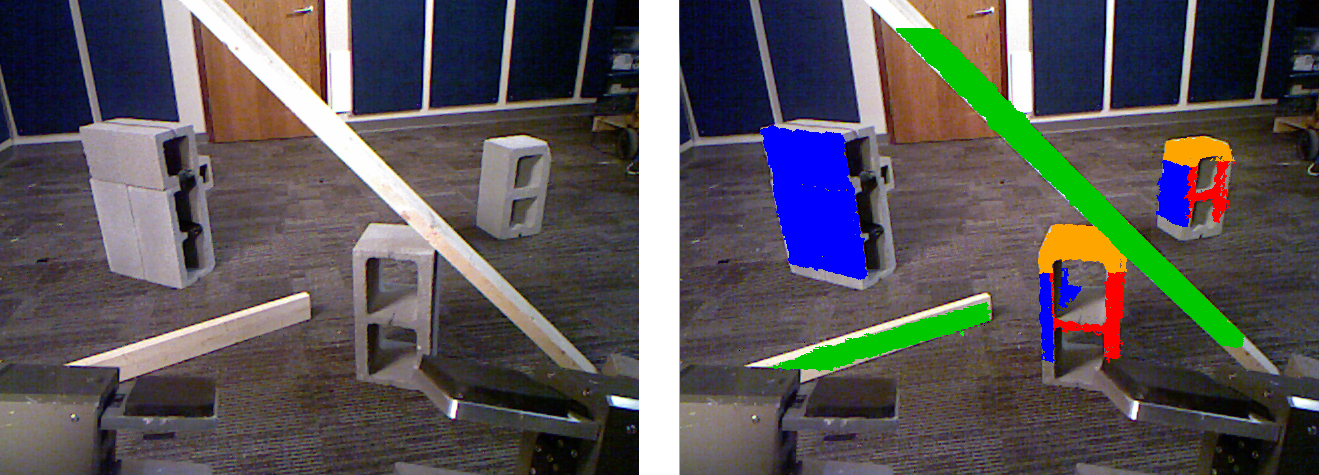
\includegraphics[width=0.9\linewidth]{Figures/detection.png}
  \caption{Cinder block and wooden plates detected as fulcrum and lever objects.}
  \label{fig:detection}
\end{figure}

The key assumption of the work is that the planner already knows the mesh of the available objects
and with minimal additional feature knowledge, such as the top of a cinder block is at 44 cm from
the ground or a lever is at least 2 meters in one dimension, we can speed up the detection. At its
current stage, the agent can autonomously detect cinder blocks, the load as shown in Figure 1, the
walls and the 2-by-4 levers. To localize objects of interest, we perform a simple scan with the tilt
and pan degrees of freedom of the RGBD camera, taking also into account the robot kinematics.

\subsection{Locomotion}

The primary locomotion strategy for Golem Krang is to balance on its two wheels, keeping its
center of mass on the vertical plane through its wheel axis. Modeled as an inverted pendulum,
locomotion via balancing has a few advantages over running on both the wheels and the back caster of
the robot. First, the footprint of the robot is smaller, 54 cm front to back due to diameter
of the wheels while dynamically balancing, as opposed to 86 cm when the robot is staticly grounded.
Second, the locomotion of the robot is simpler to model since the fixed caster without omnidirectional
wheels has different ground friction properties as the robot spins, moves forward and backward. 

The position and posture control is implemented using a proportional derivative controller based on
the inertial readings that indicate the robot angle from the vertical and the wheel encoders. In
this work, we assume the environment is setup such that the locomotion can be carried out by
turning towards the goal position, moving forward and adjusting for the goal orientation - ignoring
collisions in the world. To move forward, we use a velocity profile with limits on minimum and maximum
acceleration and deceleration. 

A significant aspect of the locomotion is the manipulation of heavy objects such as 15 kg cinder
blocks and 10 kg wooden plates. To enable stable dynamic balancing, the force-torque sensors
at the end-effectors of Golem Krang are used to incorporate the mass of the carried objects into
the robot model and update the center of mass position appropriately using forward kinematics. We
provide additional insights on heavy object manipulation in the experiments section, specifically
on the effect of the object inertia and mass on the system stability. 

\subsection{Manipulation}

The manipulation of multiple objects under motor and perception uncertainty requires a series of 
robust strategies both algorithmicly and in practical implementation. In this work, a wide range of
motion planning tools are adopted such as rapidly-expanding random trees (RRTs) \cite{kuffner2000rrt},
analytical inverse kinematics \cite{tolani2000real} and Jacobian control \cite{whitney1969resolved}. 
Additionally, to handle perception errors, we propose using guarded moves \cite{bejczy1977effect} 
that control the manipulator behavior until a predetermined tactile feedback is received. Moreover,
we deploy ``conformant motion'' behaviors where the robot action forces itself
and its environment to a desired state without any sensory feedback \cite{goldman1996expressive}. 
% 
\subsubsection{Motion planning}

Figure \ref{fig:manipulation} depicts the analytical inverse kinematics and the motion planning
steps during the manipulation of a cinder block to be used as a fulcrum. We use a predetermined
grasp location, the top surface with the holes at the sides (see Figure \ref{fig:manipulation}a).
Having observed the object and moved its base to a desirable configuration, the goal for Golem
Krang is to use one of its manipulators to grasp the object. To do so, we first use analytical
inverse kinematics to find configurations close to the object we can reach without collisions.
Figure \ref{fig:manipulation}a displays three configurations out of which the left most,
semi-transparent one collides with one of the wheels. Once a goal in arm jointspace is determined,
bidirectional RRTs with path shortening and smoothing are used to move the arm from its initial 
pose to the goal. Figure \ref{fig:manipulation}b demonstrates the keyframes as the left arm moves
around the cinder block to avoid collisions until it reaches the goal pose (green) in front of the grasp point. 

\begin{figure}[ht!] 
  \centering
  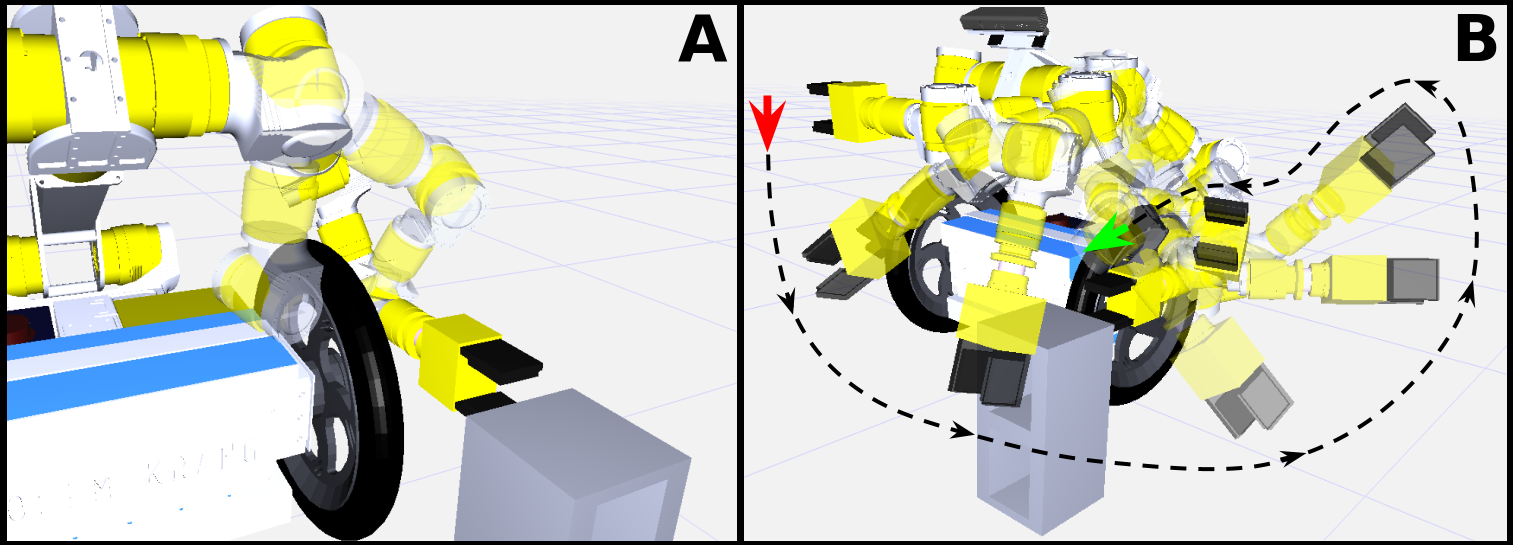
\includegraphics[width=1.0\linewidth]{Figures/manipulation.png}
  \caption{Left: Candidate grasp poses for the block - left most in collision with wheel.
  Right: RRT trajectory to goal grasp pose, moving around the block to avoid collisions.}
  \label{fig:manipulation}
\end{figure}

\vspace{-2em}
\subsubsection{Guarded and conformant motions}

Once in position using motion planning, Golem Krang uses force/torque feedback at the end-effectors
to reach out to the cinder block until contact and ensure its grippers can grasp it. Such guarded
moves have proven to be simple, heuristic alternatives to visual servoing as the robot picks up
levers, and positions them on the fulcrum and inside the load.

In addition to guarded moves with sensory feedback, we also utilize conformant motions where
in order to localize the lever more precisely, the robot runs its wheels against the lever,
usually one of them first, turning its base flush against it and eliminating any visual positioning error.
Such motions have been used before to eliminate uncertainty in the initial configuration of manipulated
objects in assembly tasks by pushing the objects into known configurations. \cite{mason1986mechanics}

\section{Experiments}

Golem Krang is tasked with overturning a 50 kg load using a lever-fulcrum assembly with a limit of
300 Nm on the force it can apply to the environment. Given the dimensions of the 
available objects in the environment, the robot has to design a structure, locate the components,
configure them into their positions and actuate the simple machine. In the following section, we
describe a typical run, focusing on details of perception, locomotion and manipulation.

Placed in a random configuration in the room, Golem Krang begins by scanning the room for the 
available objects and find the closest cinder block that would be used as a fulcrum (see Figure \ref{fig:typical_a}).
The scanning process is composed of a set of atomic behaviors which allow the robot to raise
its torso while sitting on the ground and move its arms out of its sight to avoid occlusions.
Once the fulcrum is located, the robot starts balancing and approaching the robot, until it 
positions itself in a predetermined distance to grasp the object. Using the motion planning tools,
such as RRTs and guarded moves, the robot grasps the cinder block at its top.

\begin{figure}[ht!] 
  \centering
  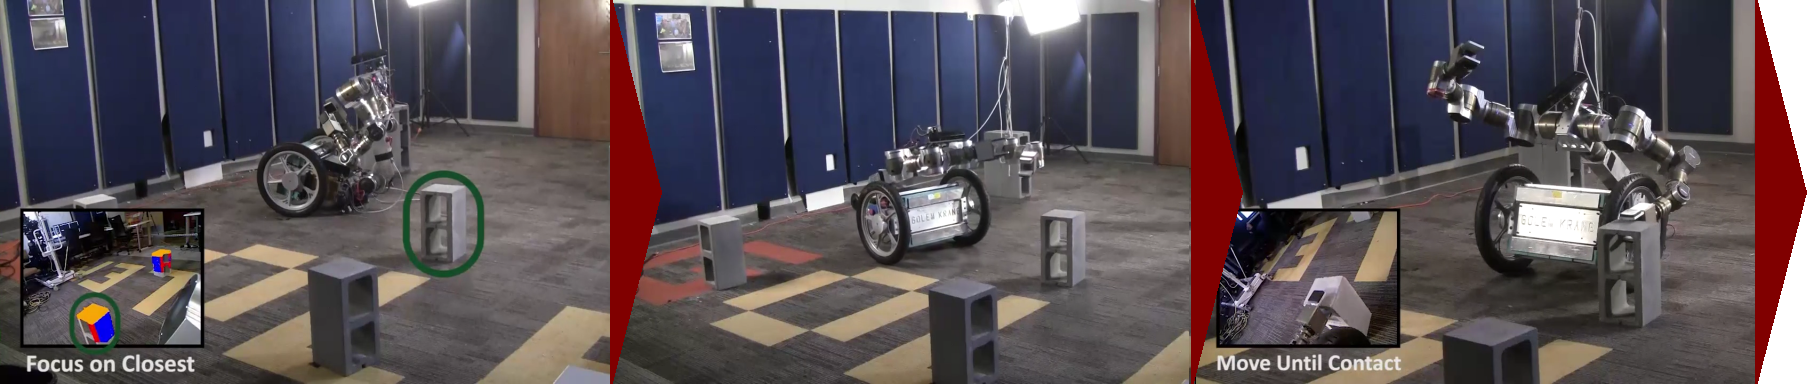
\includegraphics[width=1.0\linewidth]{Figures/a.png}
  \caption{Once Golem Krang detects the closest cinder block (left), it approaches (middle) and grasps
  the objects (right). Scene continues in Figure \ref{fig:typical_b}.}
  \label{fig:typical_a}
\end{figure}

An interesting observation we expand on in Section 4 is about how the location of a manipulated object
and the uneven distribution of its weight over the wheels affect the locomotion accuracy. To minimize
such an artifact, in Figure \ref{fig:typical_b}, Golem Krang first moves the grasped cinder block 
to the middle of its torso before turning around and localizing the load object at 50 kg. Having
detected the load, the final configuration of the fulcrum is deduced from the assembly design and
the robot places it appropriately. 

\begin{figure}[ht!] 
  \centering
  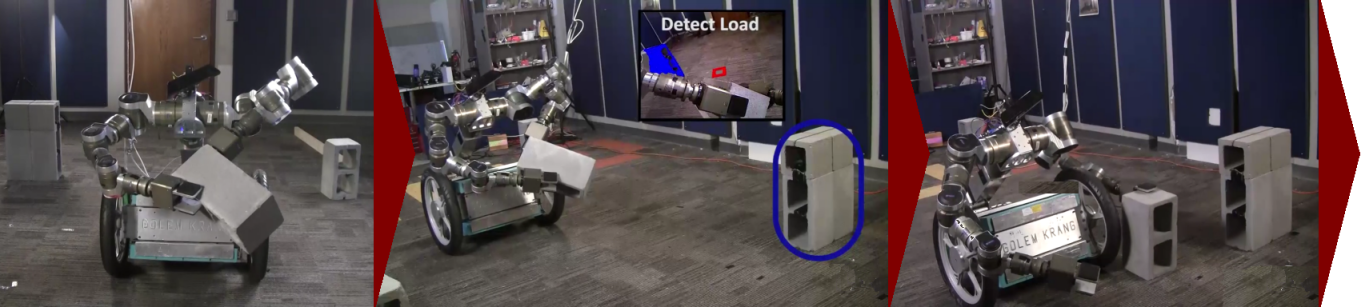
\includegraphics[width=1.0\linewidth]{Figures/b.png}
  \caption{Having grasped the fulcrum, the robot localizes the load and places the fulcrum
		in the initial design configuration. Scene continues in Figure \ref{fig:typical_c}.} 
	\label{fig:typical_b}
\end{figure}

In the third part of the experiment, Golem Krang needs to detect and localize a candidate lever
object and grasp it, as shown in Figure \ref{fig:typical_c}. Given the size of the lever and the
noisy perception data, we propose using the wheels to localize the lever object more accurately
once the robot approaches it. Figure \ref{fig:typical_c}b displays the conformant behavior where the 
robot moves forward slowly to collide with the lever and have its localization error fixed. The
left wheel first makes contact and the contact overcomes the input torque, while the right wheel 
keeps moving until the robot is parallel and directly in front of the lever. 

\begin{figure}[ht!]  	
  \centering
  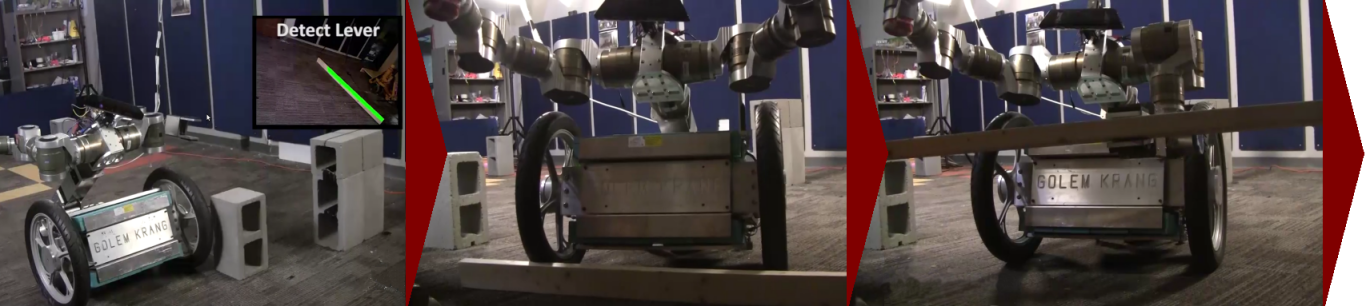
\includegraphics[width=1.0\linewidth]{Figures/c.png}
  \caption{The lever is picked up by first using vision and then running
	the wheels against the object to make physical contact before manipulation. Scene continues 
	in Figure \ref{fig:typical_d}.}
  \label{fig:typical_c}
\end{figure}

To simplify the locomotion, we have assumed collision-free paths and when Golem Krang carries the
lever, we ensure that the lever is carried high enough that it does not collide with other objects
(see Figure \ref{fig:typical_d}. Once the robot repositions itself in front of the robot, using
guarded moves, the robot first pushes the lever against the load horizontal to ensure it is at
the correct horizontal distance and then raises it until the design specification. Once at the
correct height, the robot releases the lever and allows it to slide on the fulcrum into the load
 - one of the more practically challenging tasks. For addition tasks, we have used task-constraint
 manipulation with online perception to minimize the errors during this routine. Finally, in
 Figure \ref{fig:typical_d}c, the robot pushes the object at the desired contact point and overturns
it.

\begin{figure}[ht!] 
  \centering
  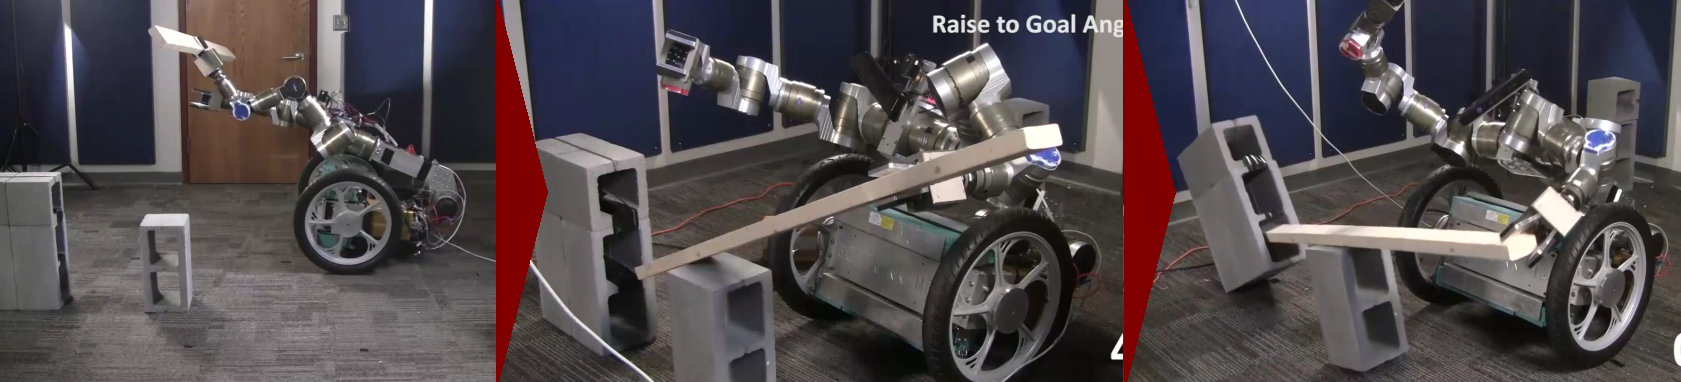
\includegraphics[width=1.0\linewidth]{Figures/d.png}
  \caption{Golem Krang places the lever in the planned pose and overturns the 50 kg load.}
  \label{fig:typical_d}
\end{figure}

\section{Results}

In this section, we provide experimental results on the functionality of the realized simple
machines under different conditions, study the sources of inaccuracies in the assembly process
and provide some insights on the autonomous manipulation of heavy objects. 

\subsubsection{Designs with Different Load Weights}

The proposed framework is tested with two 
load sizes, 50 kg and 100 kg, where the planner chooses from two levers 1.7 and 2.5
m long. Once the design is made, Golem Krang autonomously constructs it, as
described in Section 3, and we measure the force/torque sensor readings at the actuating arm gripper. Figure \ref{fig:graphs}a demonstrates the maximum applied forces at 242.27 Nm and 368.63 Nm for 50 kg and 100 kg experiments
respectively. We conclude that the mechanical advantage is 2.02:1 and 2.66:1 for each case, and 
the maximum force limit is preserved; and thus, the planned design, its assembly and actuation are
successful.

\begin{figure}[ht!] 
  \centering
  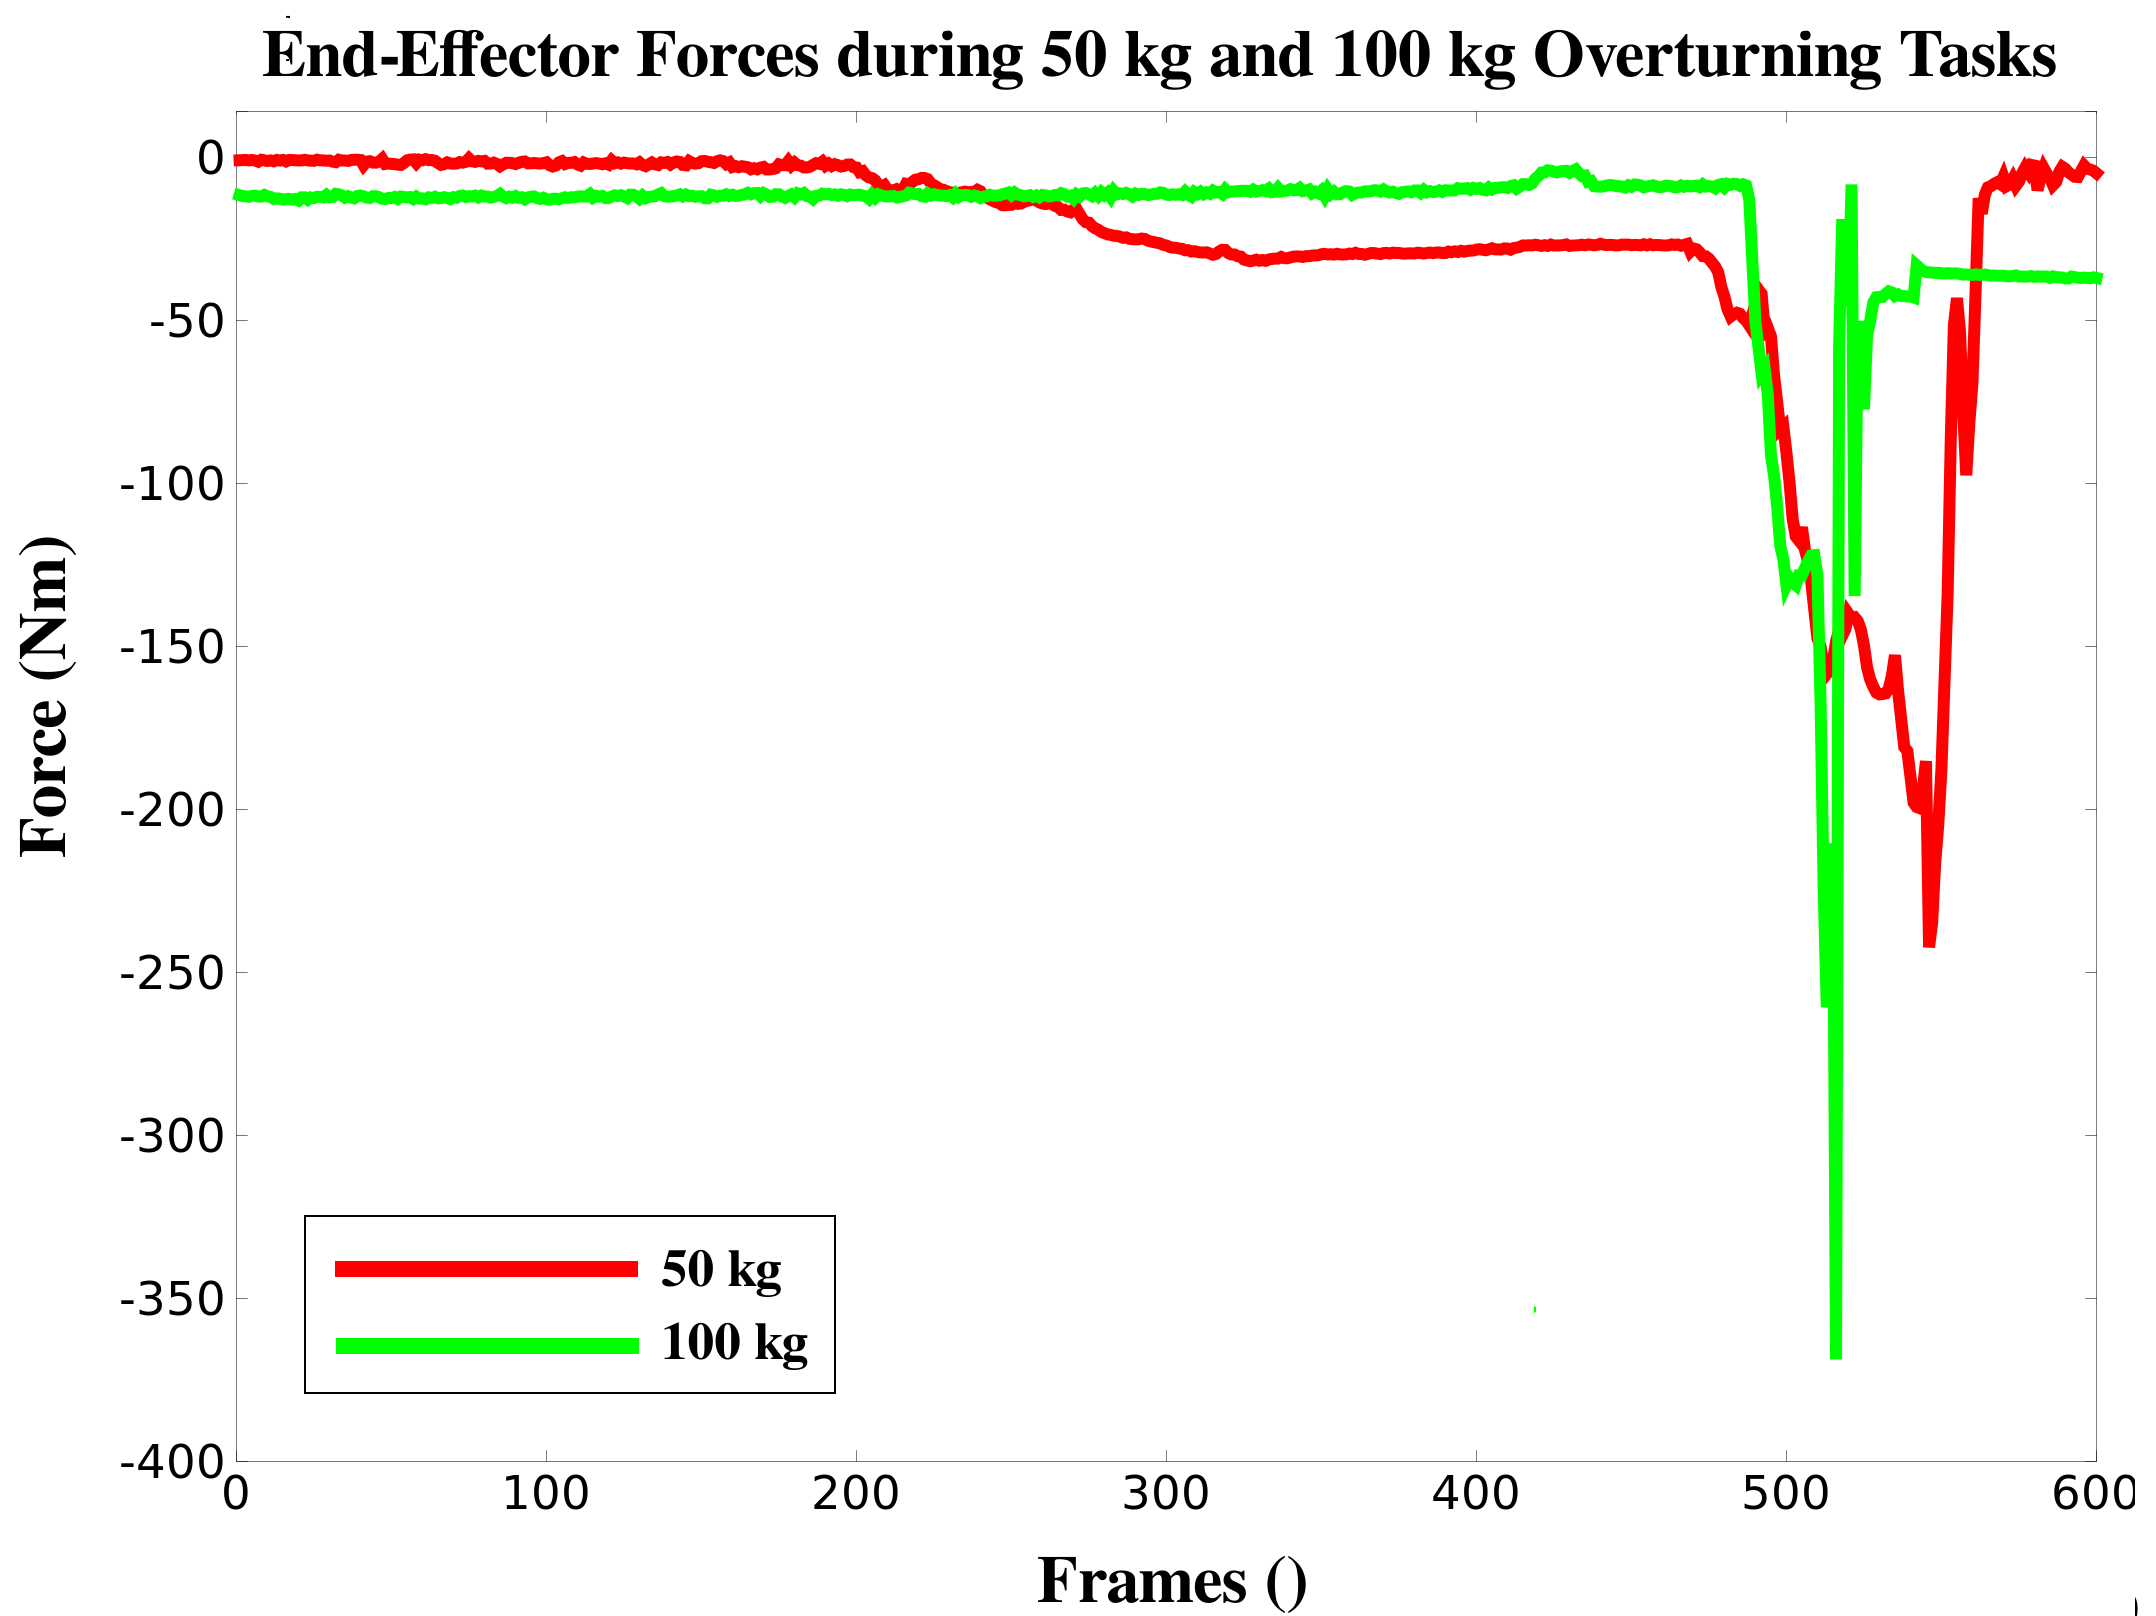
\includegraphics[width=1.0\linewidth]{Figures/loads.png}
  \caption{Left: Input forces during the 50 kg (red) and 100 kg (red) overturning tasks. 
  Right: Fulcrum shift while using a small lever leads to increased input force  (grey line).}
  
  \label{fig:graphs}
\end{figure}

\vspace{-2em}
\subsubsection{Fulcrum Base Choice and Unmodeled Implications}

The proposed planner focuses on the initial moment of force application and ensures that the force
induces enough torque to overturn the load. Although constraints are used to guarantee that the
motion is collision-free, the possibility of the the contact between
the lever and the cinder block moving is not considered. Figure \ref{fig:short}a demonstrates a case where
the planner \textit{autonomously} adapts the fulcrum base choice to accommodate the short
lever. However, the fulcrum point moves (Figures \ref{fig:short}b-c) because the contact height is
shorter than the center of mass of the load. Figure \ref{fig:graphs}b displays the increase in
the required force as the fulcrum shifts.


\begin{figure}[ht!] 
  \centering
  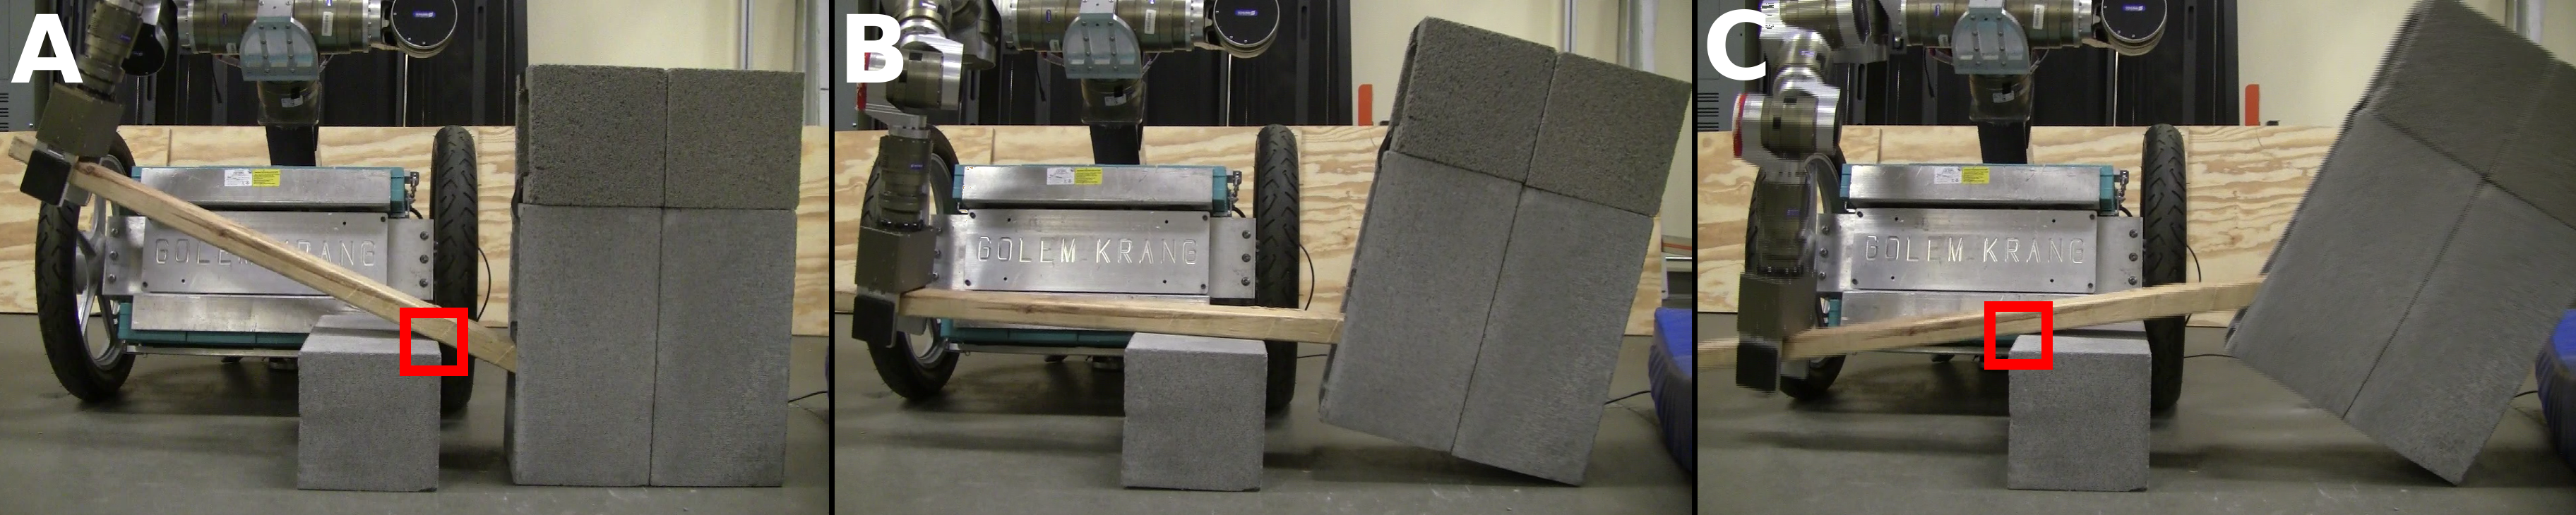
\includegraphics[width=1.0\linewidth]{Figures/short.png}
  \caption{The movement of the fulcrum-lever contact point for short lever objects.}
  \label{fig:short}
\end{figure}

\subsubsection{Evaluating Accuracy}

A challenge in long-term manipulation tasks is the accumulation of error over the course of the
executions. To remedy such an error build-up, at the current state of our work, the authors
intervene and instruct the robot to minimize its error if necessary. One of the main causes of this
inaccuracy is the reliability of the RGBD data. We observe that a mean error of 2-3 cm within a 1 m
bound increases up to 10 cm with 4 meters. The proportional increase in error with respect to
distance suggest a camera calibration problem which can be addressed with bundle adjustment \cite{pradeep2014calibrating}. 
 
Secondly, locomotion for heavy balancing robots is an active research area and our implementation
with a proportional-derivative controller can be improved following techniques as presented in
\cite{ha1996trajectory}. A major challenge is the system modeling, specifically accurate center of
mass and inertia information. Figure \ref{fig:controller} demonstrates the behavior of the robot as
it follows a velocity profile, moving straight. The sinusoidal behavior in the output position
trajectory (red) is the robot regaining its balance and the steady state error may be accommodated
with an integral term in the controller. A concern is the high-frequency velocity sinusoids which may cause instability when heavy objects are manipulated.

\begin{figure}[ht!] 
  \centering
  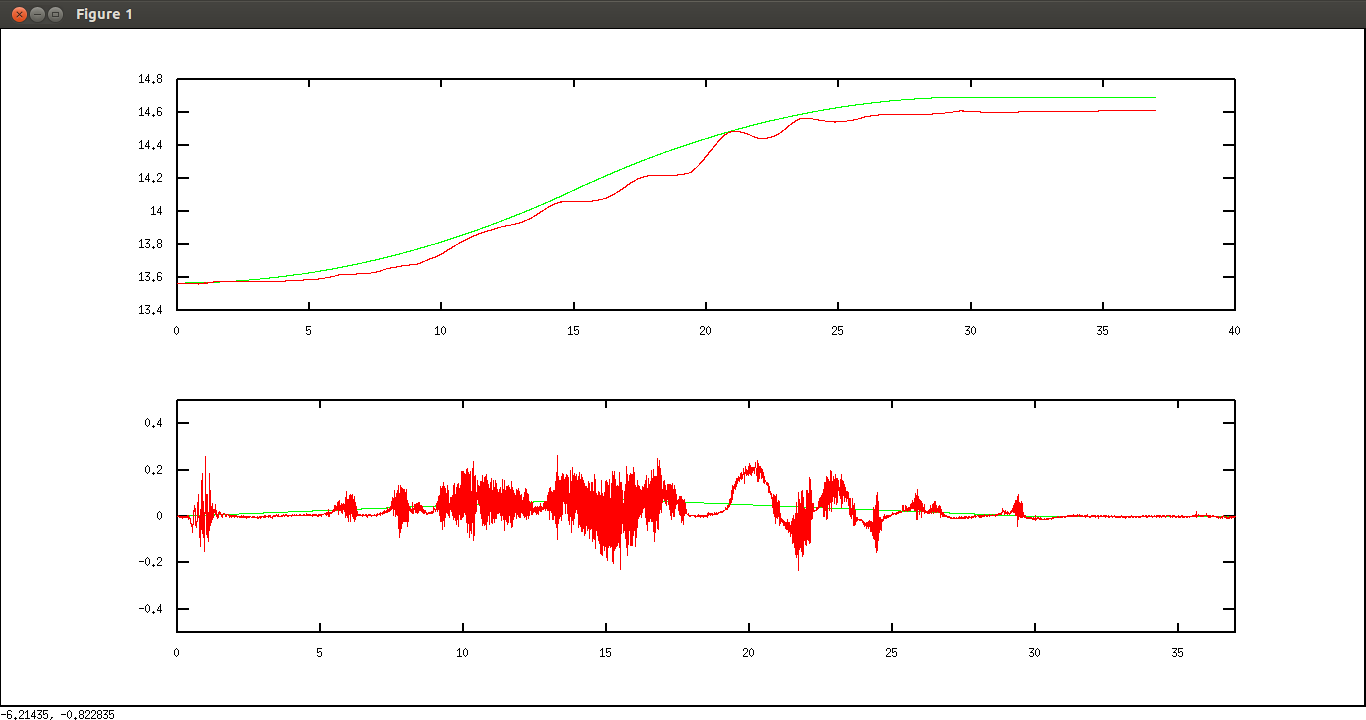
\includegraphics[width=0.9\linewidth]{Figures/controller.png}
  \caption{The oscillations and steady state error in following a reference velocity profile.}
  \label{fig:controller}
\end{figure}

\subsubsection{Manipulation of Heavy Objects}

We offer two insights from our experiments. First, the manipulation of heavy objects brings about
interesting challenges. If the object inertia model is not known, the system can be thrown off
balance easily. Moreover, when the mass of the object is mostly on one of the wheels, the robot can
start spinning since one wheel has to accommodate the extra weight. 

\newpage
% \bibliographystyle{unsrt}
% \bibliography{references}

\begin{thebibliography}{27}

\bibitem{erdogan2013planning} Erdogan, C., Stilman, M: Planning in constraint space: Automated design of
functional structures. ICRA, 2013.
\bibitem{erdogan2014incorporating} Erdogan, C., Stilman, M: Incorporating kinodynamic constraints in automated
design of simple machines. IROS, 2014.
\bibitem{vidal2006branching} Vincent, V., Geffner, H.: Branching and pruning: An optimal temporal pocl planner
based on constraint programming. AI, 2006.
\bibitem{yu2011make} Yu, L. F., Yeung, S. K., Tang, C. K., Terzopoulos, D., Chan, T. F., Osher, S: Make it home:
automatic optim. of furniture arrangement. In Siggraph, 2011.
\bibitem{beetz2010cram} Beetz, M., Mosenlechner, L., Tenorth, M: Crama cognitive robot
abstract machine for everyday manipulation in human environments. In IROS,
2010.
\bibitem{stilman2005navigation} Stilman, M., Kuffner, J. J.: Navigation among movable obstacles: Real-
time reasoning in complex environments. IJHR, 2005.
\bibitem{kemp2007challenges} Kemp, C. C., Edsinger, A., Torres-Jara, E: Challenges for robot
manipulation in human environments. IEEE Robotics and Automation Magazine,
14(1):20, 2007.
\bibitem{kuindersma2009dexterous} Kuindersma, S. R., Hannigan, E., Ruiken, D., and Grupen, R. A:
Dexterous mobility with the ubot-5 mobile manipulator. ICAR, 2009.
\bibitem{srinivasa2010herb}  Srinivasa, S. S., Ferguson, D., Helfrich, C. J., Berenson, D., 
Collet, A., Diankov, R., Gallagher, R., Hollinger, G., Kuffner, J., and
Weghe, M. V.. Herb: a home exploring robotic butler. Autonomous Robots,
28(1):5–20, 2010.
\bibitem{nishiwaki2000design} Nishiwaki, K., Sugihara, T., Kagami, S., Kanehiro, F.,
Inaba, M., and Inoue, H.: Design and development of research platform for perception-action 
integration in humanoid robot: H6. IROS, 2000.
\bibitem{dasgupta1999making} Dasgupta, A., Nakamura, Y.: Making feasible walking motion of
humanoid robots from human motion capture data. ICRA, 1999.
\bibitem{yamauchi2004packbot} Yamauchi, M. B.: Packbot: a versatile platform for military robotics. In Defense
and Security, pages 228–237. International Society for Optics and Photonics, 2004.
\bibitem{saranli2001rhex} Saranli, U., Buehler, M., Koditschek, D. E.. Rhex: A simple and
highly mobile hexapod robot. IJRR, 2001.
\bibitem{newell1961gps} Newell, A., Simon, H.: GPS, a program that simulates human thought.
DTIC, '61.
\bibitem{mccarthy1963programs} McCarthy, J.: Programs with common sense. DTIC, 1963.
\bibitem{fulkerson1961network} Fulkerson, D. R.: A network flow computation for project cost curves. Management science, 7(2):167–178, 1961.
\bibitem{taha1975integer} Taha, H.A.: Integer programming: theory, applications, and computations,
volume 975. Academic Press New York, 1975.
\bibitem{fikes1972strips} Fikes, R. E., Nilsson, N. J.: Strips: A new approach to the application of
theorem proving to problem solving. Artificial intelligence, 2(3):189–208, 1972.
\bibitem{stilman2010golem} Stilman, M., Olson, J., Gloss, W.: Golem krang: Dynamically stable
humanoid robot for mobile manipulation. ICRA, 2010.
\bibitem{kuffner2000rrt} Kuffner J.J., LaValle, S.M.: RRT-connect: An efficient approach to single-
query path planning. In ICRA. IEEE, 2000.
\bibitem{tolani2000real} Tolani, D., Goswami, A., Badler, N. I.: Real-time inverse kinematics techniques for anthropomorphic limbs. Graphical models, 62(5):353–388,
2000.
\bibitem{whitney1969resolved} Whitney, D. E.: Resolved motion rate control of manipulators and human pros-
theses. IEEE Transactions on man-machine systems, 1969.
\bibitem{bejczy1977effect} Bejczy, A.K.: Effect of hand-based sensors on manipulator control performance.
Mechanism and Machine Theory, 12(5):547–567, 1977.
\bibitem{goldman1996expressive} Goldman, R., Boddy, M.: Expressive planning and explicit knowledge. AIPS, 1996.
\bibitem{mason1986mechanics} Mason, M.T.: Mechanics and planning of manipulator pushing operations.
The International Journal of Robotics Research, 5(3):53–71, 1986.
\bibitem{pradeep2014calibrating} Pradeep, V., Konolige, K., Berger, E.: Calibrating a multi-arm multi-
sensor robot: A bundle adjustment approach. In Experimental Robotics, 1999.
\bibitem{ha1996trajectory} Ha, Y., Yuta, S.: Trajectory tracking control for navigation of the
inverse pendulum type self-contained mobile robot. Robotics and autonomous systems, 1996.

\end{thebibliography}

\end{document}

% DISCUSSION: CHALLENGES WITH VISUAL SERVOING A NONHOLONOMIC ROBOT BASE

% Having chosen the objects and their roles, the autonomous planner needs to find configurations
% for the assembly components to satisfy a range of constraints. First, the proposed assembly needs
% to be physically stable (e.g. all center of masses of upper layers within support polygons) and 
% collision-free. Second, the structure should satisfy its purpose, such as overturning a load,
% while taking into account the actuator robot's kinodynamic limitations, possibly guided by design
% principles such as the input arm of a lever being longer than the load arm for mechanical advantage.
% Note that in considering the robot limitations, we focus on the initial moment of actuation where
% presumably the required force input is maximal and output a robot configuration and required joint
% torques along with the design that is sufficient to realize the task. 
